\documentclass[a4paper, twocolumn]{article}

\usepackage{colortbl}
\usepackage{cancel}
\usepackage{siunitx}
\usepackage{multirow}
\usepackage{array}
\usepackage[table, xcdraw, dvipsnames]{xcolor}
\usepackage{times}
\usepackage{tikz}
\usepackage[top=0.75in, bottom=1in, inner=0.75in, outer=0.75in,
            headheight=45pt, headsep=2pt, footskip=5mm]{geometry}
\usepackage{graphicx}
\usepackage{anyfontsize}
\usepackage{fancyhdr}
\usepackage{indentfirst}
\usepackage{amsmath}
\usepackage[spanish, es-tabla]{babel}
\usepackage[utf8]{inputenc}
\usepackage[explicit]{titlesec}
\usepackage{etoolbox}
\usepackage{enumitem}
\usepackage[labelformat=simple,labelsep=none]{caption}
\usepackage{mathptmx}
\usepackage{lastpage}
\usepackage{pythontex}
\usepackage{booktabs}
\usepackage{amsfonts}
\usepackage[version=4]{mhchem}
\usepackage{float}
\usepackage{circuitikz}
\usepackage{subcaption}
\usepackage{changepage}
\usepackage{eso-pic}
% \usepackage{showframe}
\usepackage{minted}
\usepackage{pgfplots}


\newcommand{\inicioCodigo}{
    \newpage
    \fancyfoot[C]{}
    \onecolumn
}

\newcommand{\finalCodigo}{
    \newpage
    \fancyfoot[C]{
        \begin{tikzpicture}[remember picture, overlay]
            \draw[gray!30, line width=0.4pt]
                (0cm, 1cm) -- (0cm, 25cm);
        \end{tikzpicture}
    }
    \twocolumn
}

\renewcommand{\theenumi}{\Roman{enumi}}
\definecolor{gold}{rgb}{1.0, 0.84, 0.0}
\newcommand{\resistencia}[4]{
    \begin{minipage}{2cm}
        \begin{center}
            \begin{tikzpicture}
                \draw(-0.4cm, -0.15cm) rectangle (0.4cm, 0.15cm);
                \fill[resistor] (-0.4cm, 0) -- (-0.5cm, 0);
                \draw (-0.4cm, 0) -- (-0.5cm, 0);
                \draw (0.4cm, 0) -- (0.5cm, 0);
                \fill[#1] (-0.35cm, -0.15cm) rectangle (-0.25cm, 0.15cm);
                \fill[#2] (-0.15cm, -0.15cm) rectangle (-0.05cm, 0.15cm);
                \fill[#3] (0.05cm, -0.15cm) rectangle (0.15cm, 0.15cm);
                \fill[#4] (0.25cm, -0.15cm) rectangle (0.35cm, 0.15cm);
            \end{tikzpicture}
        \end{center}
    \end{minipage}
}
\newcommand{\diodoSilicio}[1]{
    \begin{minipage}{2cm}
        \begin{center}
            \begin{circuitikz}[scale=0.5]
                \draw[line width=1pt] (-2,0) -- (-1,0);
                \draw[line width=1pt] (2,0) -- (1,0);

                \filldraw[fill=black!75, draw=black] (-1, -0.5) rectangle (1, 0.5);

                \fill[gray!60] (0.6, -0.5) rectangle (0.8, 0.5);

                \node at (0, -1) {\texttt{#1}};
            \end{circuitikz}
        \end{center}
    \end{minipage}
}
\newcommand{\diodoGermanio}[1]{
    \begin{minipage}{2cm} 
        \begin{center}
            \begin{circuitikz}[scale=0.5]
                \draw[line width=0.8pt] (-2.5,0) -- (-1.5,0);
                \draw[line width=0.8pt] (2.5,0) -- (1.5,0);

                \filldraw[fill=white, draw=black] (-1.5, -0.4) rectangle (1.5, 0.4);
                \fill[orange!80] (-1.5, -0.25) rectangle (1.5, 0.25);
                \fill[gray!95] (1.2, -0.4) rectangle (1.5, 0.4);
                \node at (0, -0.9) {\texttt{#1}};
            \end{circuitikz}
        \end{center}
    \end{minipage}
}
\newcommand{\inv}[1]{\frac{1}{#1}}
\newcommand{\recuadrar}[2]{
    \begin{center}
        \begin{tabular}{|m{#1}|}
            \toprule
            \multicolumn{1}{|c|}{\hspace{5pt}#2\hspace{5pt}} \\
            \bottomrule
        \end{tabular}
    \end{center}
}

\newcommand{\ecuacion}[1]{
    \begin{center}
        $#1$
    \end{center}
}

\newcommand{\longsection}[2]{%
    \section[#1]{\parbox{\columnwidth}{#1}}
}

\newcommand{\saltoPag}[0]{%
    \newpage\noindent\thispagestyle{fancy}%
    \begin{tikzpicture}[remember picture, overlay]
        \draw[line width=0.4pt, color=gray!50] (8.5cm, -0.4cm) -- (8.5cm, -24cm);
    \end{tikzpicture}%
    \ignorespaces{}
}

\newcommand{\midTitle}[2]{%
    \begin{center}
        \textcolor{#1}{\underline{#2}} 
    \end{center}
}

\captionsetup{
    format=hang,
    labelfont={bf},
    textfont=normalfont,
    labelsep=colon,
    justification=centering,
    singlelinecheck=true
}

\newcommand{\imagen}[3][]{
    \begin{center}
        \begin{tikzpicture}
            \node[inner sep=2pt] (image) {\includegraphics[width=#2]{#3}};
            \draw[line width=1pt, color={rgb:red,251;green,73;blue,52}] (image.south west) rectangle (image.north east);
        \end{tikzpicture}
        \ifx\\#1\\
            \captionof{figure}{}
        \else
            \captionof{figure}{#1}
        \fi 
        \label{fig:#2}
    \end{center}
}

\newcommand{\sangria}[0]{\par\noindent\hspace*{15pt}}

\newcommand{\longsubsection}[2]{%
    \subsection[#1]{\parbox{\columnwidth}{#1}}%
}

\begin{document}
    \author{}\date{}\title{}
\thispagestyle{empty}
\begin{tikzpicture}[remember picture, overlay]
    \pgftransformshift{\pgfpoint{0cm}{0cm}}
    \draw [line width=2pt](1cm,-1cm) -- (1cm,-27.7cm) -- (14cm, -27.7cm) -- (14cm, -1cm) -- (1cm, -1cm);
    \draw[line width=2pt] (15cm, -27.7cm) -- (19cm,-27.7cm) -- (19cm, -1cm) -- (15cm, -1cm) --  (15cm, -27.7cm);
    \node [line width=2pt] at (17cm, -3.5cm) {
\includegraphics[width=3cm]{./imagenes/utn.png}};
	\node [line width=2pt] at (7.5cm, -9cm) {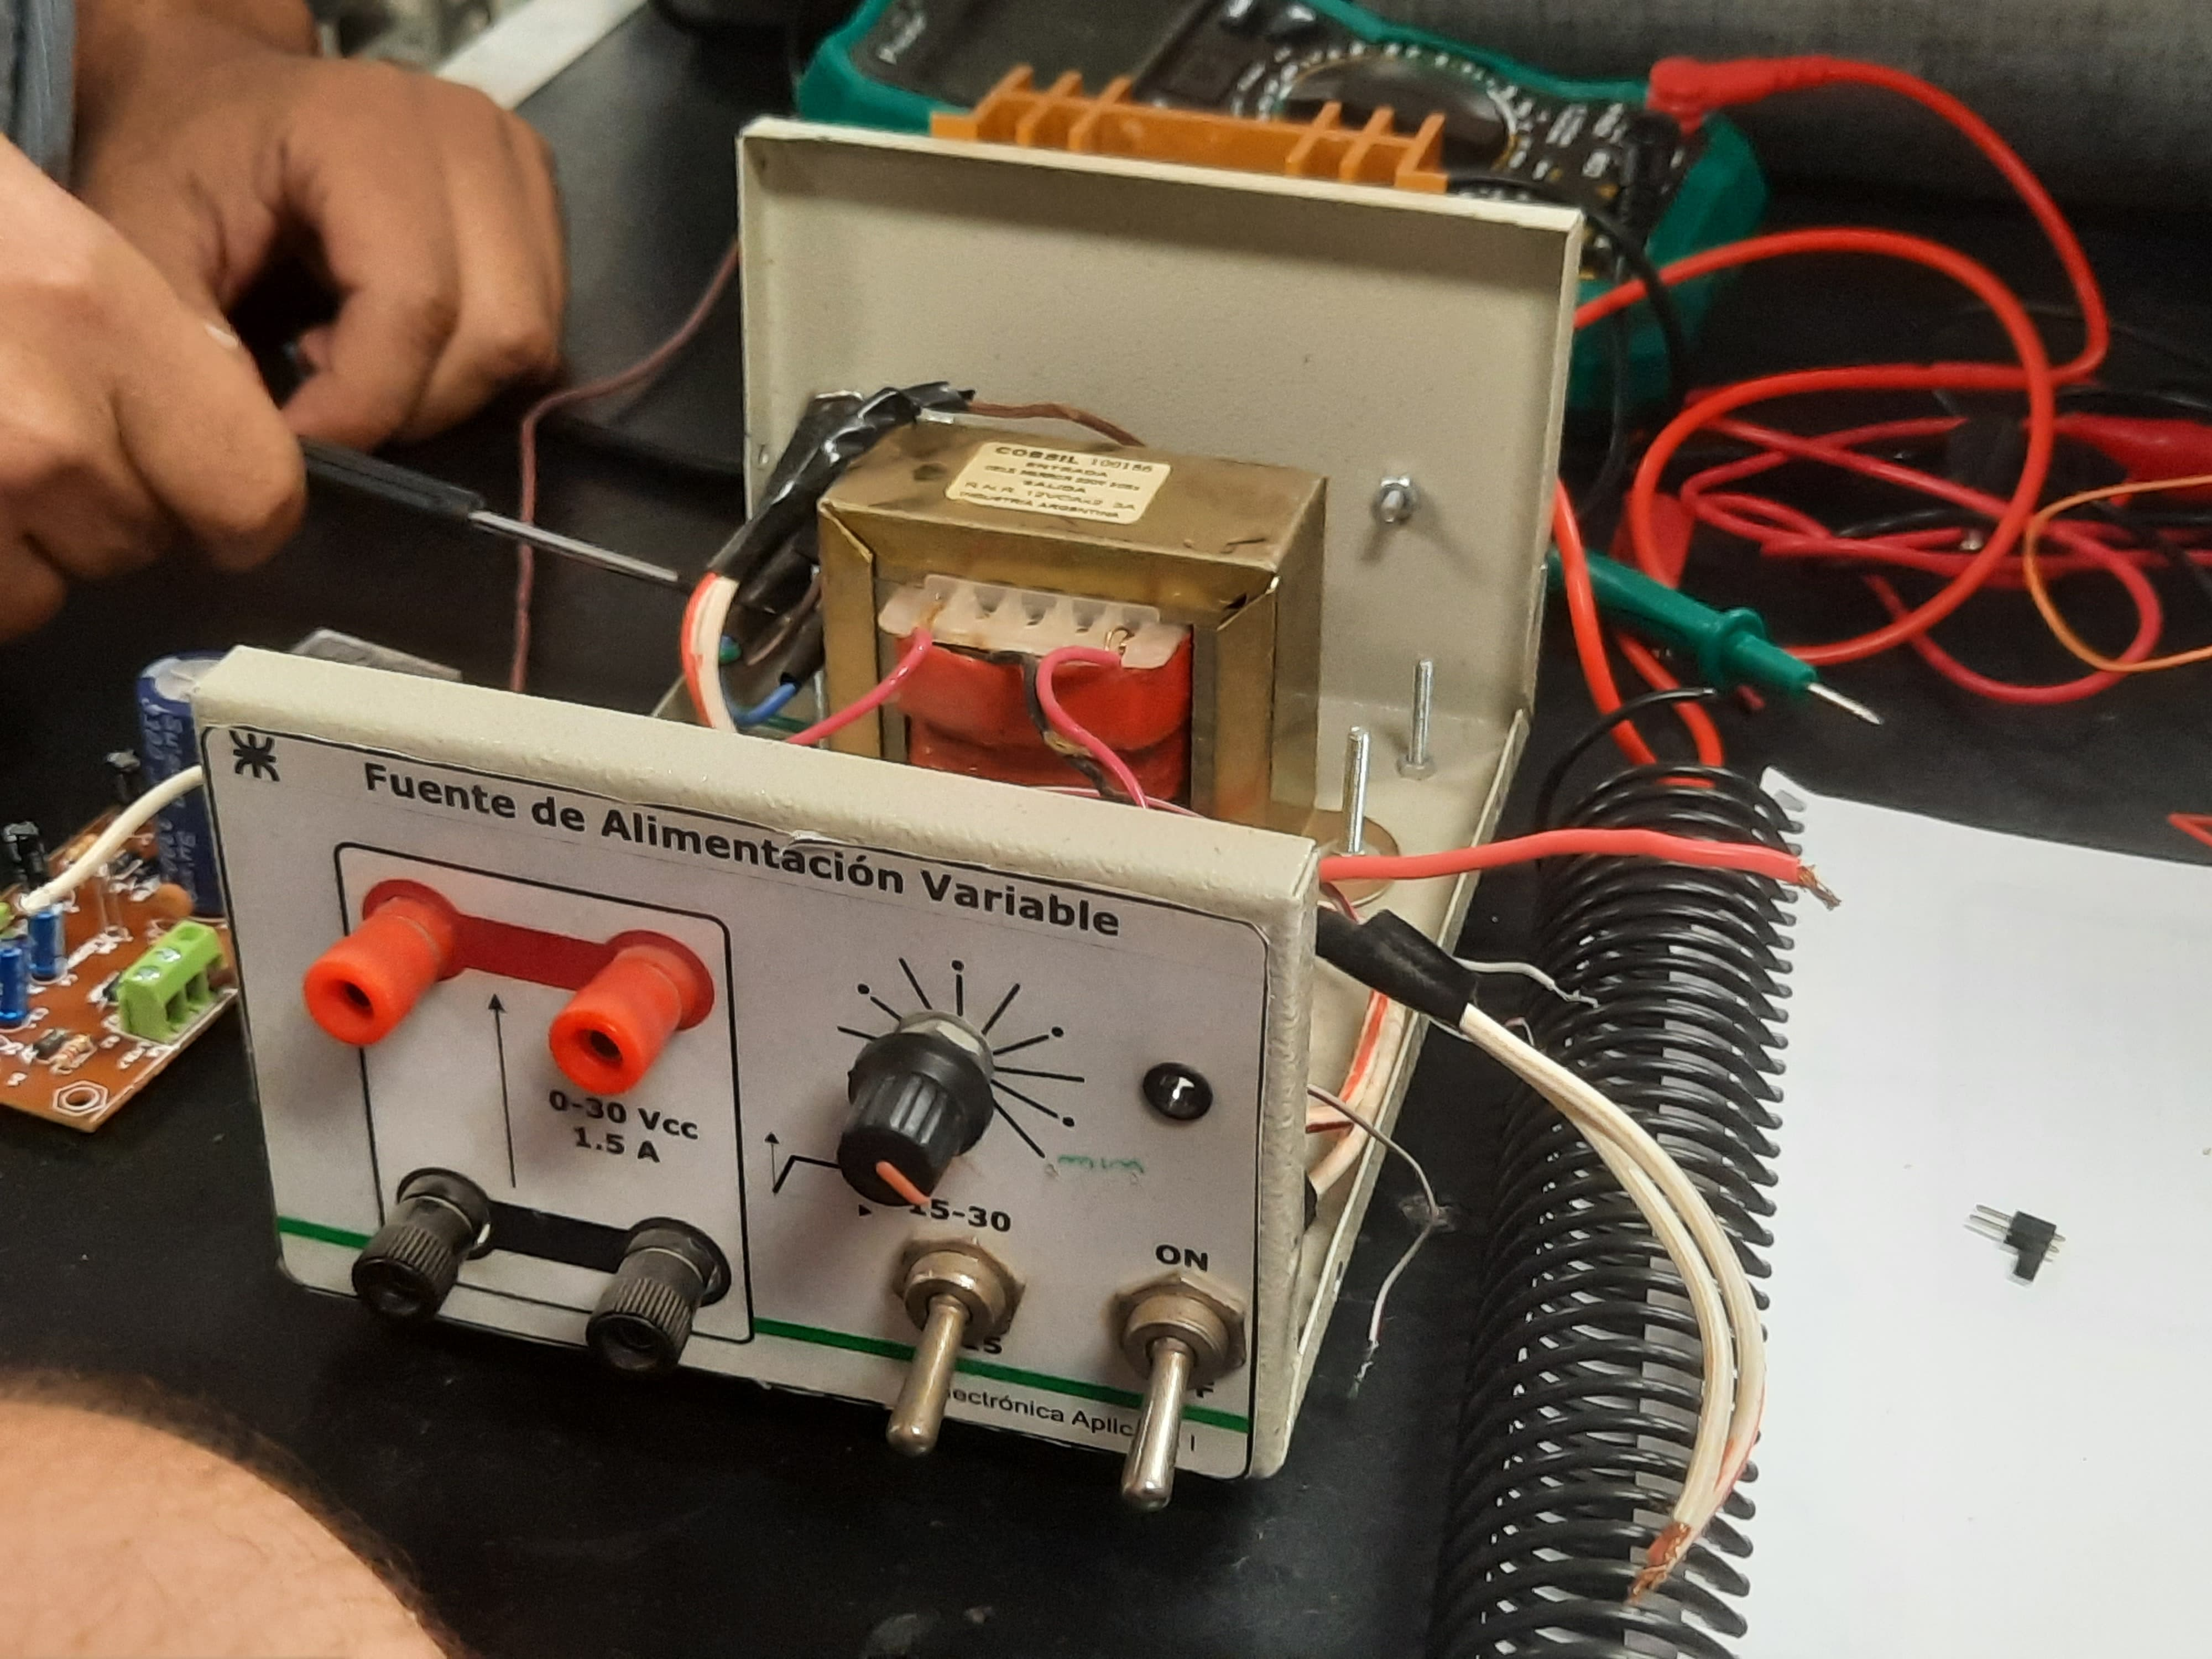
\includegraphics[width=8cm]{./imagenes/portada.jpg}};
    \node at (17cm, -7cm) {\scalebox{5}{\textbf{U}}};
    \node at (17cm, -9cm) {\scalebox{5}{\textbf{T}}};
    \node at (17cm, -11cm) {\scalebox{5}{\textbf{N}}};
    \node at (17cm, -14cm) {\scalebox{5}{\textbf{F}}};
    \node at (17cm, -16cm) {\scalebox{5}{\textbf{R}}};
    \node at (17cm, -18cm) {\scalebox{5}{\textbf{C}}};
    \node at (7.5cm, -14cm) {\scalebox{3}{\textbf{TP N° 2}}};
    \node at (7.5cm, -15cm) {\scalebox{3}{\textbf{Diodos}}};
    \node at (7.5cm, -16cm) {\scalebox{3}{\textbf{Zener y Recortadores}}}; 
    \node at (7.5cm, -23.5cm) {
	\begin{minipage}[c]{12cm}
	    \begin{itemize}
            \raggedright
            \item \fontsize{12}{12}\selectfont \textbf{Autores:} 
                \begin{itemize} \item Gonzalo Ezequiel Filsinger - Leg. 403797  \item Ignacio Ismael Perea - Leg. 106265 \item Mariano Alberto Condori - Leg. \item Marcos Acevedo - Leg.   \end{itemize}
            \item \fontsize{12}{12}\selectfont \textbf{Curso:} 3R1  \\
            \item \fontsize{12}{12}\selectfont \textbf{Asignatura:} Dispositivos Electrónicos.
            \item \fontsize{12}{12}\selectfont \textbf{Institución:} Universidad Tecnológica Nacional - Facultad Regional de Córdoba.
        \end{itemize}
    \end{minipage}};
\end{tikzpicture}
    \renewcommand{\headrulewidth}{0.4pt}
\renewcommand{\footrulewidth}{0.4pt}
\definecolor{textoGris}{HTML}{222222}

\fancypagestyle{fancy}{
    \fancyhf{}

    \fancyfoot[R]{[Filsinger G. - Perea I. - Condori M. - Acevedo M.] [\textbf{pág.\ \thepage} de \pageref{LastPage}]}

    \fancyfoot[C]{
        \begin{tikzpicture}[remember picture, overlay]
            \draw[gray!30, line width=0.4pt]
                (0cm, 1cm) -- (0cm, 25cm);
        \end{tikzpicture}
    }

    \fancyhead[L]{
        \begin{tabular}{@{}l@{}}
            \raisebox{-0.5\height}{
\includegraphics[height=0.60in]{./imagenes/logoDepartamentoElectronica.png}}
            \begin{tabular}{@{}l@{}}
                {\color{textoGris}\textbf{Departamento de Ingeniería Electrónica}} \\
                {\color{textoGris}Facultad Regional Córdoba}
            \end{tabular}
        \end{tabular}
    }
}
\titleformat{\section}[hang]{\fontsize{10}{12}\bfseries}{\thesection.}{0.5em}{\underline{#1}}
\titleformat{\subsection}[hang]{\fontsize{10}{11}\bfseries}{\thesubsection.}{0.5em}{#1}
\titleformat{\subsubsection}[hang]{\fontsize{10}{10}\itshape}{\thesubsubsection.}{0.5em}{#1}
\widowpenalty=10000
\clubpenalty=10000
\enlargethispage{-1cm}
    \newpage\thispagestyle{empty}\text{}\newpage\newpage\thispagestyle{empty}\setcounter{page}{0}\tableofcontents\newpage\newpage\thispagestyle{empty}\text{}\setcounter{page}{0}
    \pagestyle{fancy}
    \section{Actividad 1: Identificacion de Pines}

\paragraph{La polaridad de los terminales del diodo está especificada en su encapsulado según lo visto en las clases de aula. De todas formas es posible validar esta polaridad con el multímetro, es justamente lo que se realizará en esta actividad.}

\subsection{Materiales usados:}
\begin{itemize}
    \item Diodo de silicio 1N4007 y diodos de germanio 1N60
    \item Multímetro
    \item Protoboard
\end{itemize}

\subsection{Mediciones:}
Primero colocamos el multimetro en modo de deteccion de diodos o continuidad. Para luego colocar los diodos en la protoboard y proceder a medirlos en un sentido y luego en el otro.

\begin{table}[h!]
\centering
\large
\setlength{\tabcolsep}{9pt}
\renewcommand{\arraystretch}{1.5}
\begin{tabular}{|c|c|c|}
\hline
\textbf{Sentido} & \textbf{Germanio} & \textbf{Silicio} \\
\hline
\parbox[c][2.5cm][c]{2.5cm}{\centering % Espacio para imagen de sentido 1
\vspace{0.2cm}
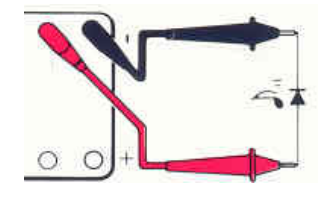
\includegraphics[width=2cm]{imagenes/sentido1.png}
\vspace{0.2cm}
} &0.312 &0.611 \\
\hline
\parbox[c][2.5cm][c]{2.5cm}{\centering % Espacio para imagen de sentido 2
\vspace{0.2cm}
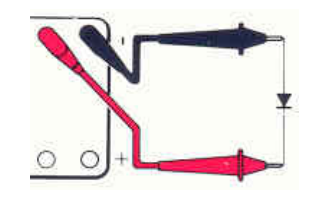
\includegraphics[width=2cm]{imagenes/sentido2.png}
\vspace{0.2cm}
} &0 &0 \\
\hline
\end{tabular}
\caption{Mediciones de diodos con multímetro}
\end{table}

\begin{figure}[h!]
    \centering
    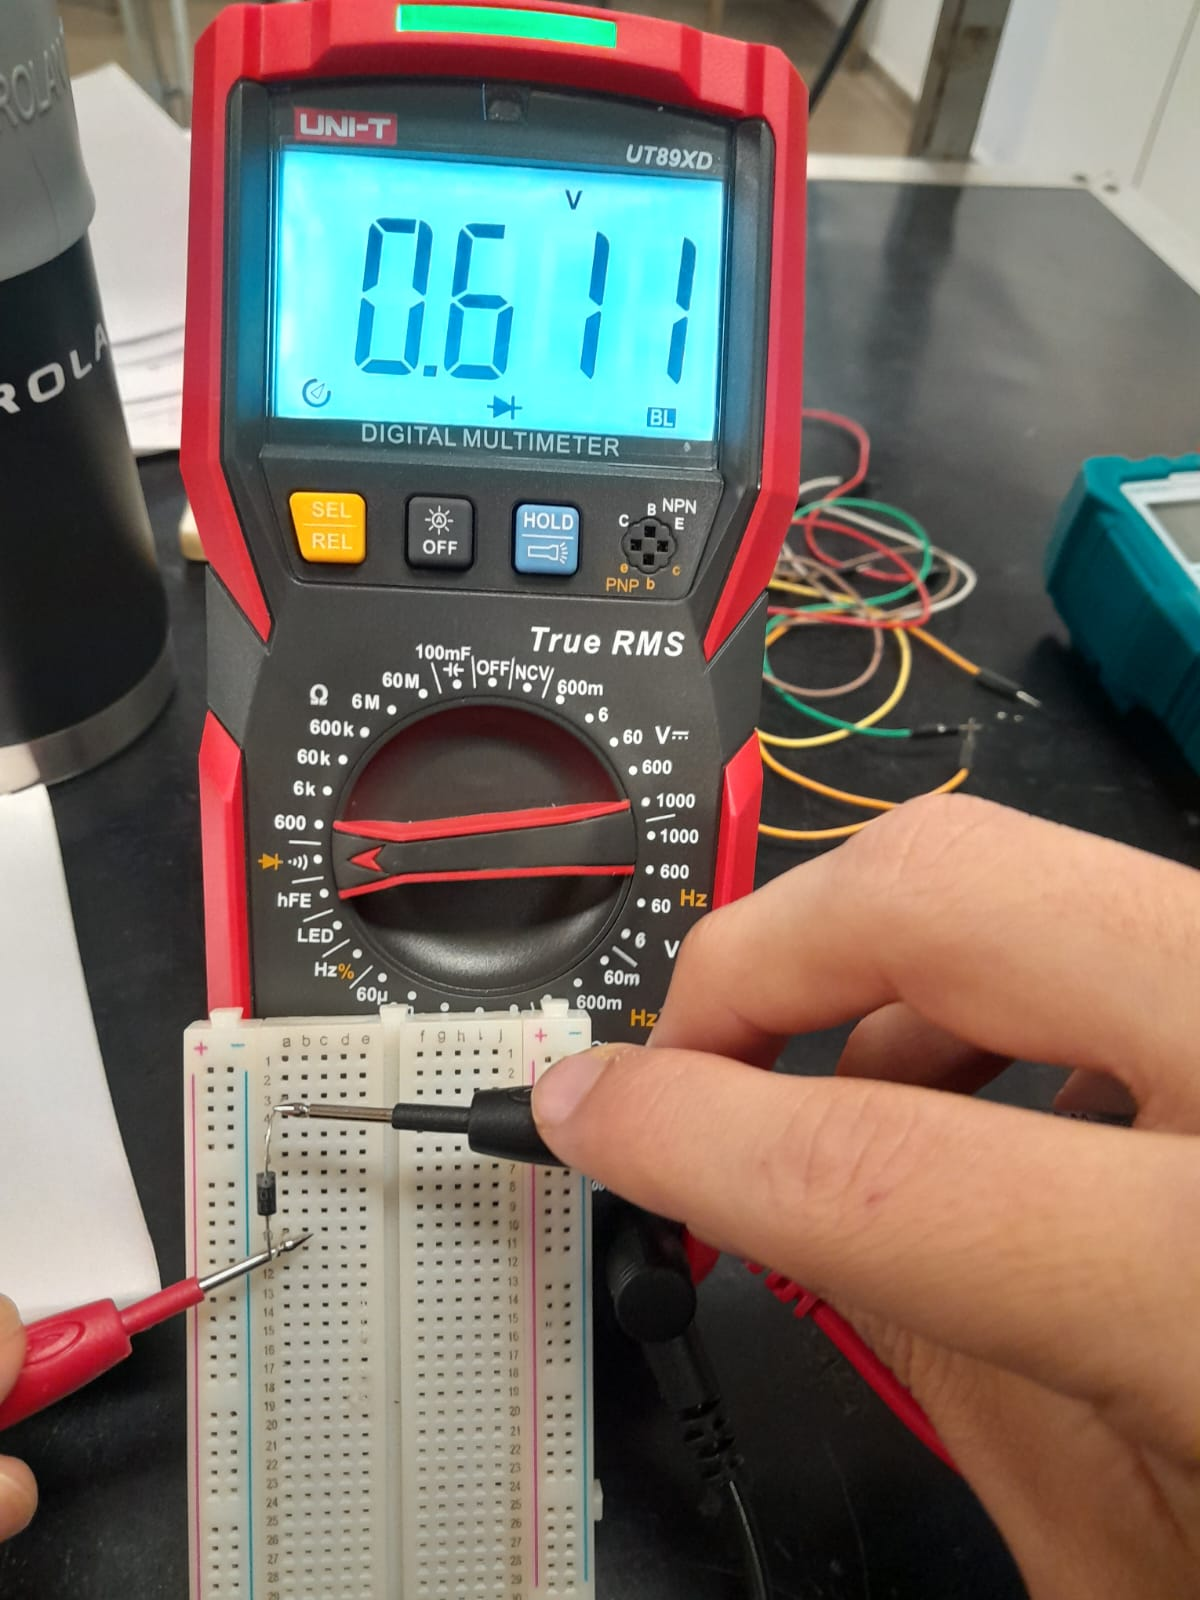
\includegraphics[width=0.45\linewidth]{imagenes/silicio_directa.jpg}
    \hspace{0.05\linewidth}
    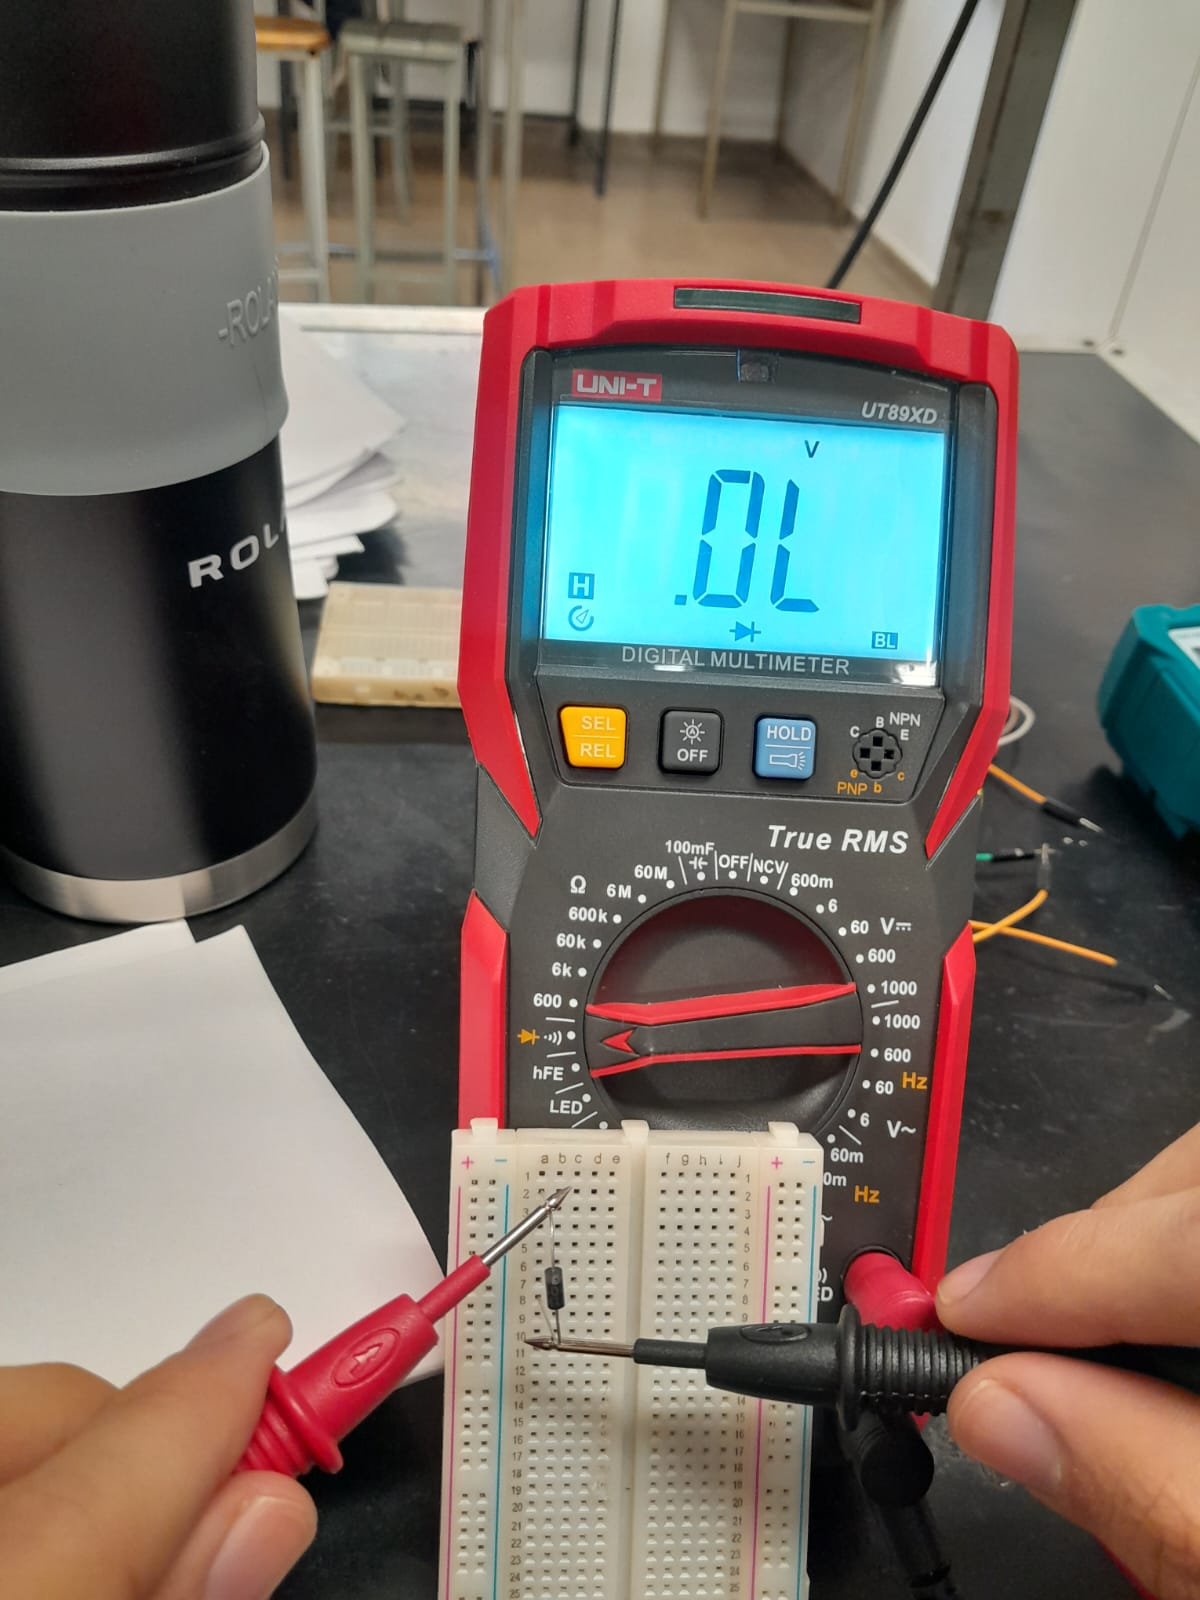
\includegraphics[width=0.45\linewidth]{imagenes/silicio_inversa.jpg}
\end{figure}

\subsection{Conclusiones}
Como se puede observar en la tabla y en las imagenes, los valores que solemos usar de 0.7 para silicio y 0.3 para germanio son solo aproximaciones ya que pudimos medir que dependiendo del diodo este varía un poco, en este caso obtuvimos 0.611 para el diodo de silicio y 0.312 para el de germanio.


    \newpage

\section{Actividad 2: Polarización de la juntura BE}


\subsection{Consigna de Laboratorio}
Armar el circuito en una plataforma de simulación con el objetivo de observar la curva de la corriente de base a medida que aumenta la tensión de polarización de la juntura base-emisor. Es importante identificar el codo de la corriente y la estabilidad de la tensión VBE una vez polarizada la juntura. Podría, sí le parece, hacer simulaciones modificando otros parámetros que en el circuito básico se encuentran fijos como VCC(V2) o la temperatura ambiente simulada.

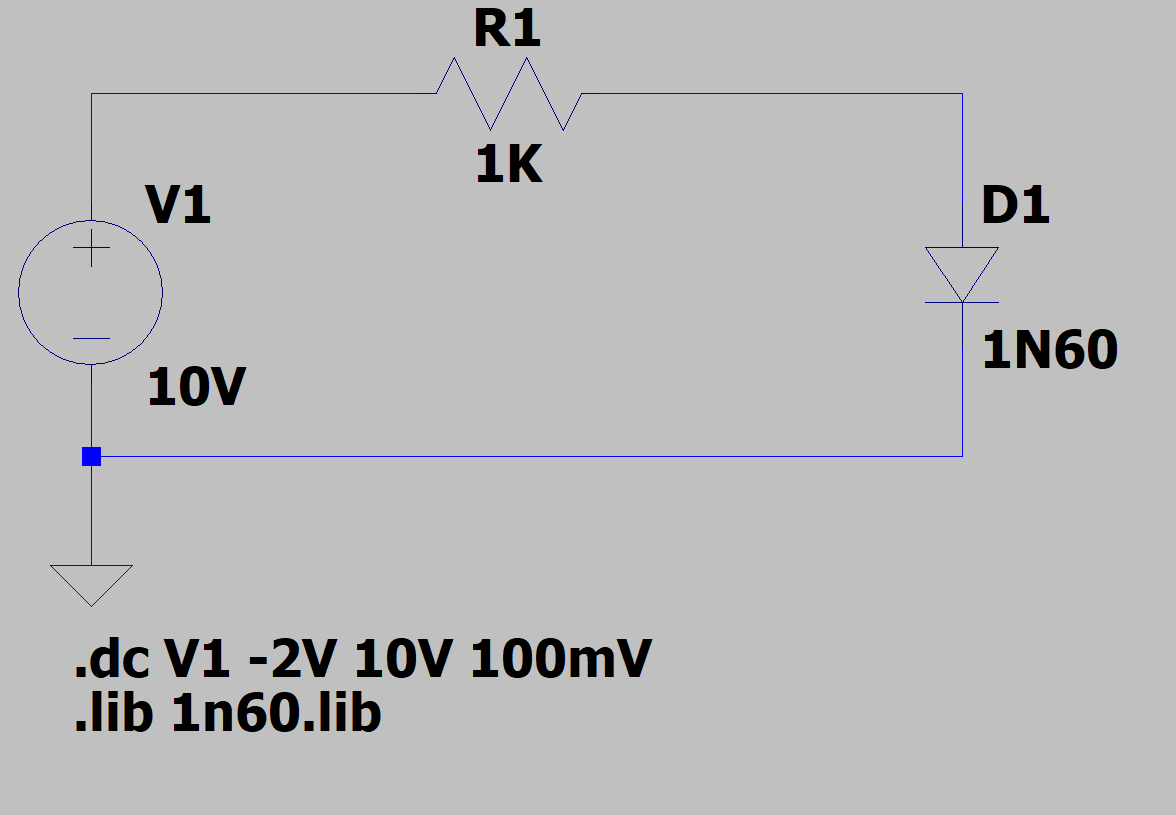
\includegraphics[width=7cm]{./imagenes/Circuito2.jpg}




\subsection{Materiales usados:}
\begin{itemize}
    \item Transistor BC546/7/8/9.
    \item Resistores $R_s = \SI{10}{\kilo\ohm}$, $R_c = \SI{560}{\ohm}$.
    \item Fuentes de alimentación.
\end{itemize}

Circuito implementado:\\

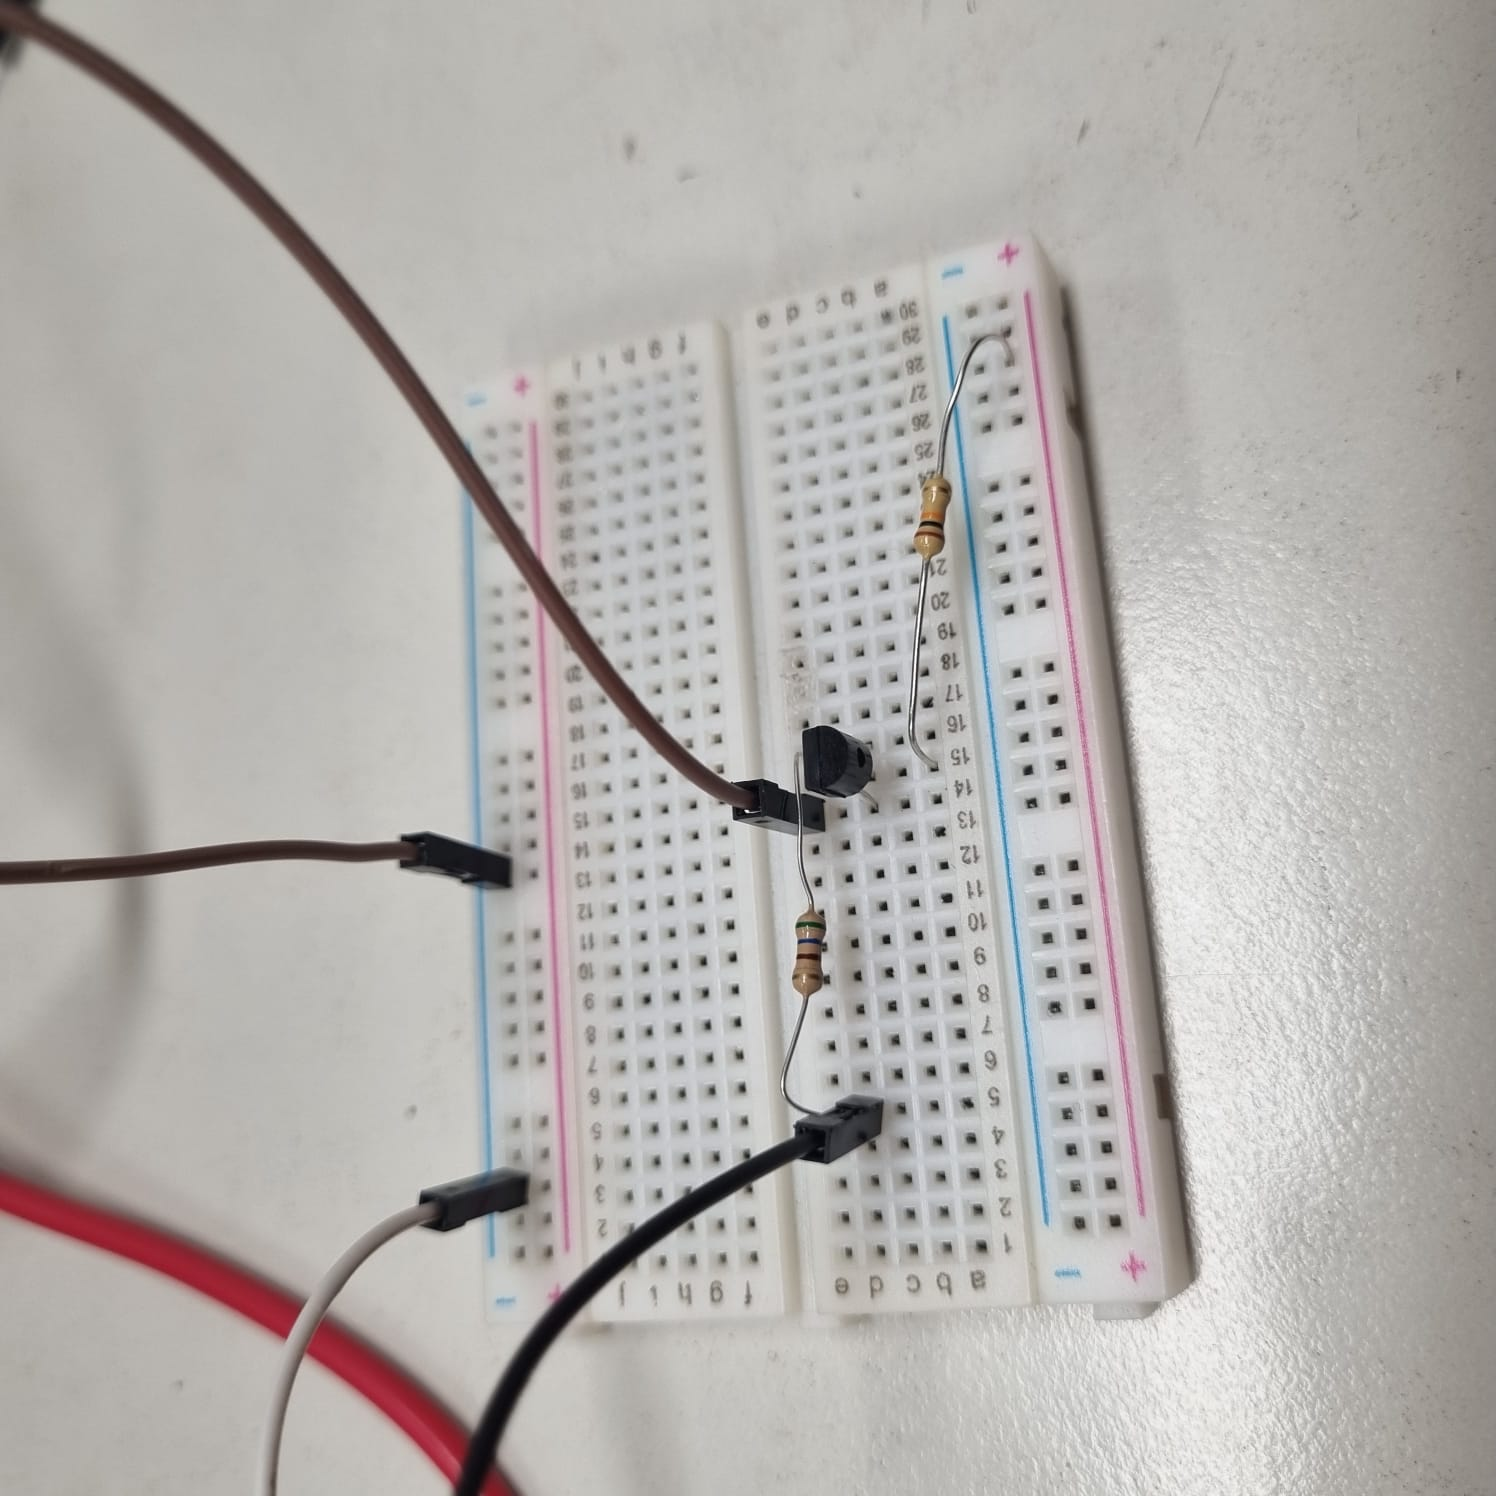
\includegraphics[width=7cm]{./imagenes/Lab1.jpg}

\newpage

\subsection{Procedimiento}

Manteniendo la $V_{CC} = 10V$, realice un barrido de $0V$ a $10V$ de $V_{BB}$. Se recomienda variar la tensión cada $100mV$ a $500mV$ dependiendo de la proximidad a la región del codo de polarización de la juntura. Aplique las recomendaciones realizadas en el anterior trabajo práctico. Debe medir: $V_{BB}$, $V_{BE}$ e $I_B$. Es importante tener en cuenta el límite de disipación de potencia tanto del transistor como del resistor $R_C$. Si bien el práctico está centrado en el comportamiento de la juntura BE, si el transistor pasa a la zona activa, permitirá corriente en $I_C$ e incrementará la potencia disipada en el resistor del colector. Puede comprobar qué sucede en el simulador y graficar la disipación de potencia en función del barrido de la fuente $V_{BB}$.

\subsection{Tabla de Mediciónes}
Mantenemos la $V_{CC} = 10V$, realizamos un barrido de 0V a 10V de $V_{BB}$ para completar la siguiente tabla:

\begin{table}[ht]
\resizebox{\columnwidth}{!}{%
\begin{tabular}{|l|l|l|l|l|l|l|}
\hline
\rowcolor[HTML]{FFFFFF} 
\cellcolor[HTML]{FFCE93}$V_{BB}$ & $500mV$      & $1V$          & $2V$        & $3V$        & $4V$        & $5V$        \\ \hline
\cellcolor[HTML]{FFCE93}$I_B$    & $4,64 \mu A$ & $30,43 \mu A$ & $124 \mu A$ & $220 \mu A$ & $323 \mu A$ & $913 \mu A$ \\ \hline
\cellcolor[HTML]{FFCE93}$V_{BE}$ & $0,493 V$    & $0,682 V$     & $0,73 V$    & $0,74 V$    & $0,74 V$    & $0,75 V$    \\ \hline
\end{tabular}%
}
\end{table}

En case a dicha tabla podemos armar el siguiente grafico:

\begin{figure}[H]
    \centering
    \resizebox{0.49\textwidth}{!}{%
    \begin{tikzpicture}
        \begin{axis}[
            xlabel={$V_{BE}$ [V]},
            ylabel={$I_B$ [$\mu$A]},
            grid=both,
            xmin=0.45, xmax=0.8,
            ymin=0, ymax=1000,
            xtick={0.5,0.6,0.7,0.75},
            ytick={0,200,400,600,800,1000},
            legend pos=north west,
        ]
        \addplot[
            color=blue,
            mark=*,
            thick
        ] coordinates {
            (0.493,4.5)
            (0.682,30.43)
            (0.73,124)
            (0.74,220)
            (0.74,323)
            (0.75,913)
        };
        \end{axis}
    \end{tikzpicture}
    }
    \caption{Curva de $I_B$ en función de $V_{BE}$}
    \label{fig:ib_vs_vbe}
\end{figure}

    \section{Circuitos recortadores con diodos zener}

\section*{Objetivo}
El objetivo de este trabajo es comprender y analizar el uso de los diodos zener en aplicaciones de corriente alterna (CA), específicamente como recortadores de voltaje, mediante la simulación y la implementación práctica de los circuitos.


\subsection*{Actividad de Simulación}
Se simuló el comportamiento de los circuitos a) y b) mostrados en la Figura 4. Estos circuitos utilizan diodos zener para limitar la señal de salida a determinados niveles de tensión.

% AQUÍ VA LA IMAGEN DE LOS CIRCUITOS a) Y b)
\begin{figure}[H]
    \centering
    %\includegraphics[width=0.8\textwidth]{ruta/circuitos_zener.png}
    \caption{Circuitos con diodos zener para recorte de tensión: a) recorte simétrico, b) recorte asimétrico.}
\end{figure}

\subsubsection*{Configuración en LTspice}
\begin{itemize}
    \item Se utilizó una fuente de 24 VCA como entrada.
    \item Se colocó una resistencia limitadora de 1 k$\Omega$ en serie.
    \item Se usaron diodos zener de:
    \begin{itemize}
        \item 5,1 V y 20 V para el circuito a).
        \item 6,8 V y 12 V para el circuito b).
    \end{itemize}
\end{itemize}

\subsubsection*{Resultados de la Simulación}
A continuación se presentan las señales de salida obtenidas para ambos circuitos simulados.

% AQUÍ VA LA IMAGEN DE LA SALIDA DEL CIRCUITO A)
\begin{figure}[H]
    \centering
    %\includegraphics[width=0.7\textwidth]{ruta/salida_circuito_a.png}
    \caption{Señal de salida del circuito a) con recorte simétrico.}
\end{figure}

% AQUÍ VA LA IMAGEN DE LA SALIDA DEL CIRCUITO B)
\begin{figure}[H]
    \centering
    %\includegraphics[width=0.7\textwidth]{ruta/salida_circuito_b.png}
    \caption{Señal de salida del circuito b) con recorte asimétrico.}
\end{figure}

\subsubsection*{Análisis}
\begin{itemize}
    \item En el circuito a), los diodos zener actúan en ambas mitades del ciclo de la señal AC, recortando los picos a aproximadamente ±5,1 V y ±20 V.
    \item En el circuito b), el recorte se realiza de forma asimétrica: uno de los semiperíodos se limita a ±6,8 V y el otro a ±12 V.
\end{itemize}

\subsection{Actividad de Laboratorio}

El objetivo de la actividad es analizar la aplicación de los diodos zener como recortadores. Para ello se implementarán los circuitos a) y b) de la Figura 4.

\textbf{Instrumental y componentes:}
\begin{enumerate}
    \item Osciloscopio
    \item Diodos Zener de 5,1 V, 6,8 V, 12 V y 20 V (todos 2W o 5W según disponibilidad)
    \item Resistencia 1 k$\Omega$ (2W)
    \item Transformador 220 VCA / 24 VCA
\end{enumerate}

\subsection*{Procedimiento}

\textbf{Paso 1: Cálculo de la resistencia limitadora de corriente}

Para limitar la corriente que circula por los diodos zener, se utiliza una resistencia en serie. El valor de esta resistencia se calcula mediante la siguiente fórmula:

\[
R = \frac{V_{\text{in(max)}} - V_Z}{I_Z + I_L}
\]

Donde:
\begin{itemize}
    \item \( V_{\text{in(max)}} \): Tensión máxima de entrada (24 VCA $\rightarrow$ $V_{pico} \approx 33.9$ V)
    \item \( V_Z \): Tensión zener del diodo correspondiente
    \item \( I_Z \): Corriente mínima de conducción del zener (se asume 5 mA)
    \item \( I_L \): Corriente de carga (se asume despreciable)
\end{itemize}

\textbf{Circuito a):}  
Zener de 5,1 V y 20 V conectados en oposición. Se usa el mayor valor (20 V):

\[
R_a = \frac{33.9 - 20}{0.005} = 2780\ \Omega
\]

\textbf{Circuito b):}  
Zener de 6,8 V y 12 V conectados en oposición. Se usa el mayor valor (12 V):

\[
R_b = \frac{33.9 - 12}{0.005} = 4380\ \Omega
\]

En ambos casos se eligió una resistencia de 1 k$\Omega$ (2W), ya que permite el funcionamiento del zener sin sobrepasar los valores de corriente seguros.

\textbf{Paso 2: Armado del circuito a)}

Se armó el circuito a) de la Figura 4 en protoboard, utilizando los componentes indicados.

% AQUÍ VA LA FOTO DEL CIRCUITO A) ARMADO
\begin{figure}[H]
    \centering
    %\includegraphics[width=0.7\textwidth]{ruta/circuito_a_fisico.png}
    \caption{Circuito a) armado en protoboard.}
\end{figure}

\textbf{Paso 3: Medición de la señal de salida del circuito a)}

Se conectó el osciloscopio a la salida y se registró la señal recortada por los zener.

% AQUÍ VA LA CAPTURA DE PANTALLA DEL OSCILOSCOPIO - CIRCUITO A)
\begin{figure}[H]
    \centering
    %\includegraphics[width=0.7\textwidth]{ruta/osciloscopio_circuito_a.png}
    \caption{Señal de salida del circuito a) medida con osciloscopio.}
\end{figure}

\textbf{Paso 4: Armado del circuito b)}

Se armó el circuito b) con los zener de 6,8 V y 12 V, usando también la resistencia de 1 k$\Omega$.

% AQUÍ VA LA FOTO DEL CIRCUITO B) ARMADO
\begin{figure}[H]
    \centering
    %\includegraphics[width=0.7\textwidth]{ruta/circuito_b_fisico.png}
    \caption{Circuito b) armado en protoboard.}
\end{figure}

\textbf{Paso 5: Medición de la señal de salida del circuito b)}

Se registró la forma de onda a la salida del circuito con el osciloscopio.

% AQUÍ VA LA CAPTURA DE PANTALLA DEL OSCILOSCOPIO - CIRCUITO B)
\begin{figure}[H]
    \centering
    %\includegraphics[width=0.7\textwidth]{ruta/osciloscopio_circuito_b.png}
    \caption{Señal de salida del circuito b) medida con osciloscopio.}
\end{figure}

\textbf{Paso 6: Comparación con la simulación}

Se compararon las señales reales obtenidas con las formas de onda obtenidas en LTspice. Se verificó buena concordancia entre los valores de tensión de recorte esperados y medidos.

\textbf{Paso 7: Conclusiones intermedias}

\begin{itemize}
    \item En el circuito a), el recorte es simétrico (±5,1 V y ±20 V).
    \item En el circuito b), el recorte es asimétrico (±6,8 V y ±12 V).
    \item El uso de diodos zener en oposición permite limitar la señal en ambas mitades del ciclo.
    \item La resistencia limitadora es fundamental para proteger los zener y controlar la corriente.
\end{itemize}
\section{Análisis sobre parámetros de hoja de datos}
    
\newpage
\section{Actividad 4: Interpretación de las especificaciones del fabricante}

\subsection{Actividad}

Para esta actividad vamos a buscar los siguientes datos en la en el datasheet del transistor seleccionado.

\begin{itemize}
    \item $I_{DSS}$:2-20mA
    \item $V_{DS}$ máx: 25V
    \item $V_{GS}$: 0 a -25V
    \item $P_{t}$ : 350 mW
    \item $V_{br}$: -25V
    \item $V_{GS(off)}$ : -8V
\end{itemize}

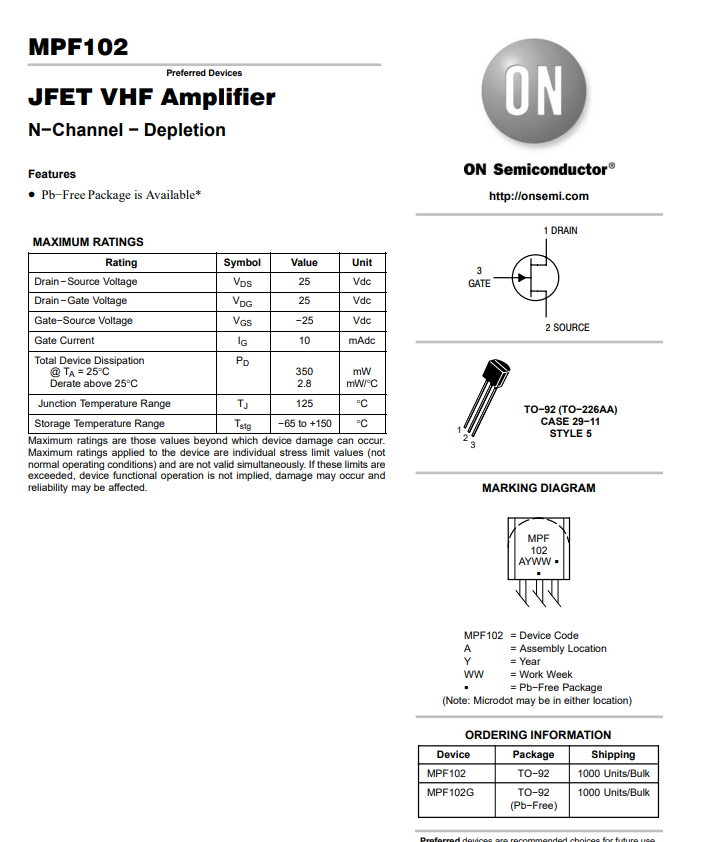
\includegraphics[width=6cm]{./imagenes/Datasheet.png}
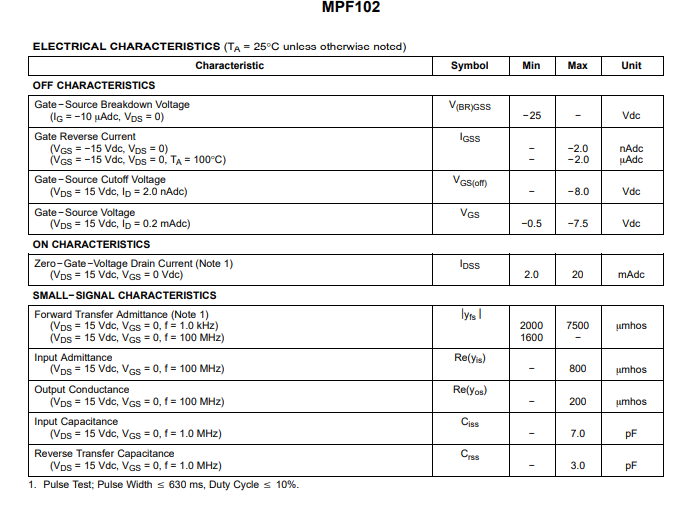
\includegraphics[width=6cm]{./imagenes/Datasheet2.png}
    \newpage

\section{Actividad 5: Interpretación de las especificaciones del fabricante}

\subsection{Actividad}

Para esta actividad vamos a buscar los siguientes datos en la en el datasheet del transistor seleccionado.

\begin{itemize}
    \item $I_{DS}$
    \item $V_{DS}$
    \item $V_{GS}$
    \item $P_{t}$
    \item $V_{br}$
    \item $V_{GS(off)}$
\end{itemize}
    \newpage

\section{Actividad 6: Control de disparo del TRIAC}
    \newpage

\section{Actividad 7: Interpretación del Datasheet}

\subsection{Parametros del DIAC}

\subsection{Parametros del SCR}

\begin{itemize}
    \item \textbf{VDRM} (Voltaje máximo directo de bloqueo): Es el voltaje máximo que el SCR puede soportar en polarización directa sin dispararse. En este caso, es de 600V.
    \item \textbf{IT(RMS)} (Corriente RMS máxima): Es la corriente máxima que el SCR puede manejar en condiciones normales de operación. En este caso, es de 4A.
    \item \textbf{IT(AV)} (Corriente media máxima): Es la corriente media máxima que el SCR puede manejar en un ciclo completo. En este caso, es de 2.55A.
    \item \textbf{ITSM} (Corriente de pulso máxima): Es la corriente máxima que el SCR puede manejar en un pulso corto. En este caso, es de 20A.
    \item \textbf{IDRM} (Corriente de fuga en bloqueo directo): Es la corriente que fluye a través del SCR cuando está en polarización directa pero no está disparado. En este caso, es de 10µA.
    \item \textbf{IGT} (Corriente de disparo): Es la corriente mínima que se debe aplicar a la compuerta para disparar el SCR. En este caso, es de 15µA la típica y 200µA la máxima.
    \item \textbf{VGT} (Voltaje de disparo): Es el voltaje mínimo que se debe aplicar a la compuerta para disparar el SCR. En este caso, es de 0.4V la mínima, 0.6V la típica y 0.8V la máxima.
    \item \textbf{IH} (Corriente de mantenimiento): Es la corriente mínima que debe fluir a través del SCR para mantenerlo en estado de conducción después de haber sido disparado. En este caso, es de 0.19mA la típica y 3mA la máxima.
    \item \textbf{tgt} (Tiempo de disparo): Es el tiempo que tarda el SCR en cambiar de estado de bloqueo a estado de conducción después de que se aplica la corriente de disparo a la compuerta. En este caso, es de 1.2µs.
    \item \textbf{tq} (Tiempo de apagado): Es el tiempo que tarda el SCR en volver al estado de bloqueo después de que la corriente a través de él cae por debajo de la corriente de mantenimiento. En este caso, es de 40µs.
    \item \textbf{R$\theta$JC} (Resistencia térmica unión a carcasa): Es la resistencia térmica entre la unión del SCR y su carcasa. En este caso, es de 3°C/W.
    \item \textbf{R$\theta$JA} (Resistencia térmica unión a ambiente): Es la resistencia térmica entre la unión del SCR y el ambiente. En este caso, es de 75°C/W.
\end{itemize}

\subsection{Parametros del TRIAC}
\end{document}